
\section{Calculations \& Graphs}

\vspace{-0.5cm}
\singlespacing

%------- Force --------%

\subsection{Momentum} 

{\centering
\begin{equation}
	p = mv 
	\label{eq:momentum}
\end{equation}
\begin{align*}
	\mathbf{p} &: \text{Momentum} \\
	\mathbf{m} &: \text{Mass of object} \\
	\mathbf{v} &: \text{Velocity of object} 
\end{align*}}

\subsubsection{Sample Calculation \\ {\normalfont \small\textit{using initial momentum of red cart in Part 1, trial 1}}}

{\centering
\begin{align*}
	p &=  mv \\
		&=  (1 \text{ kg})(5 \text{ m/s}) \\ 
	p &= \boxed{5 \text{ kg m/s}} 
\end{align*}}

%------- ACCELERATION BETWEEN TWO POINTS WITH INITIAL VELOCITY CLOSE TO ZERO--------%

\subsection{Kinetic Energy} 

{\centering
\begin{equation}
	\text{KE} = \frac{1}{2}mv^2 
	\label{eq:energyK}
\end{equation}
\begin{align*}
	\boldsymbol{m} &: \text{mass} \\
	\boldsymbol{v} &: \text{velocity} 
\end{align*}}

\subsubsection{Sample Calculation \\ {\normalfont \small\textit{initial kinetic energy of red cart, part 1 trial 2}}}

\begin{align*}
	\text{KE} &= \frac{1}{2}mv^2 \\ \\
										&= \frac{1}{2}(1 \text{ kg})(5 \text{ m/s})^2 \\ \\
	\text{KE} &= \boxed{12.5\,\text{J}}
\end{align*}

\newpage
%------- ACCELERATION BETWEEN TWO POINTS --------%

%------- AVERAGE VALUE --------%
%------- AVERAGE VALUE --------%

%------- STANDARD DEVIATION --------%
%------- STANDARD DEVIATION --------%

%------- RELATIVE ERROR --------%
\subsection{Percent Difference Between Change Calculated Momentum and Impulse From Graph}
\vspace{0.5cm}
\begin{equation}
	\text{PD}	= \left| \frac{\text{measured - actual}}{\text{actual}} \right|\: \text{x}\: 100\%
	\label{eq:pdiff}
\end{equation}

\subsubsection{Sample Calculation \\ {\normalfont \small\textit{using values from part 3}}}

\begin{align*}
	\text{PD}	&= \left| \frac{\text{measured - actual}}{\text{actual}} \right|\: \text{x}\: 100\% \\ \\
	\text{PD}	&= \left| \frac{\text{0.4933 - 0.4724}}{\text{0.4724}} \right|\: \text{x}\: 100\% \\ \\
			PD &= \boxed{4.431\%} 
\end{align*}
%------- RELATIVE ERROR --------%
\newpage
%----TABLES-----%
%----TABLES-----

\subsection{Tables}
\begin{table}[H]
\captionsetup{font=Large}
\caption{Part 1: Elastic Collisions - Pre Collision}
\resizebox{\textwidth}{!}{%
\begin{tabular}{@{}ccccc@{}}
\toprule
\textbf{Trial}                                   & 1    & 2    & 3  & 4  \\ \midrule
\textbf{Red Cart Mass (kg)}                      & 1    & 1    & 1  & 2  \\
\textbf{Blue Cart Mass (kg)}                     & 1    & 2    & 1  & 1  \\
$\textbf{Red Cart }\mathbf{V_o}\textbf{ (m/s)}$  & 5    & 5    & 5  & 5  \\
$\textbf{Blue Cart }\mathbf{V_o}\textbf{ (m/s)}$ & 0    & 0    & -3 & 0  \\
\textbf{Total Momentum (kg m/s)}                 & 5    & 5    & 2  & 10 \\
\textbf{Total KE (J)}                            & 12.5 & 12.5 & 17 & 25 \\ \bottomrule
\label{tab:part1pre}
\end{tabular}%
}
\end{table}

\begin{table}[H]
\captionsetup{font=Large}
\caption{Part 1: Elastic Collisions - Post Collision}
\resizebox{\textwidth}{!}{%
\begin{tabular}{@{}ccccc@{}}
\toprule
\textbf{Trial}                                     & 1    & 2    & 3  & 4    \\ \midrule
\textbf{Red Cart Mass (kg)}                        & 1    & 1    & 1  & 2    \\
\textbf{Blue Cart Mass (kg)}                       & 1    & 2    & 1  & 1    \\
$\textbf{Red Cart   }\mathbf{V_f}\textbf{ (m/s)}$  & 0    & -1.7 & -3 & 1.7  \\
$\textbf{Blue Cart   }\mathbf{V_f}\textbf{ (m/s)}$ & 5    & 3.3  & 5  & 6.7  \\
\textbf{Total Momentum (kg m/s)}                   & 5    & 4.9  & 2  & 10.1 \\
\textbf{Total KE (J)}                              & 12.5 & 12.3 & 17 & 25.3 \\ \midrule
\textbf{Total Momentum \% Difference (\%)}         & 0    & 2    & 0  & 1    \\
\textbf{KE \% Difference (\%)}                     & 0    & 1.32 & 0  & 1.34 \\ \bottomrule
\label{tab:part1post}
\end{tabular}%
}
\end{table}

\begin{table}[H]
\centering
	\captionsetup{font=Large}
\caption{Part 2: Inelastic Collisions - Pre Collision}
\label{tab:part2pre}
\resizebox{10cm}{!}{%
\begin{tabular}{@{}ccc@{}}
\toprule
\textbf{Trial}                                     & 1  & 2  \\ \midrule
\textbf{Red Cart Mass (kg)}                        & 1  & 1  \\
\textbf{Blue Cart Mass (kg)}                       & 1  & 3  \\
$\textbf{Red Cart   }\mathbf{V_o}\textbf{ (m/s)}$  & 6  & 6  \\
$\textbf{Blue Cart   }\mathbf{V_o}\textbf{ (m/s)}$ & 0  & 0  \\
\textbf{Total Momentum (kg m/s)}                   & 6  & 6  \\
\textbf{Total KE (J)}                              & 18 & 18 \\ \bottomrule
\end{tabular}%
}
\end{table}

\begin{table}[H]
\centering
\captionsetup{font=Large}
\caption{Part 2: Inelastic Collisions - Post Collision}
\label{tab:part2post}
\resizebox{10cm}{!}{%
\begin{tabular}{@{}ccc@{}}
\toprule
\textbf{Trial}                                     & 1  & 2   \\ \midrule
\textbf{Red Cart Mass (kg)}                        & 1  & 1   \\
\textbf{Blue Cart Mass (kg)}                       & 1  & 3   \\
$\textbf{Red Cart   }\mathbf{V_f}\textbf{ (m/s)}$  & 3  & 1.5 \\
$\textbf{Blue Cart   }\mathbf{V_f}\textbf{ (m/s)}$ & 3  & 1.5 \\
\textbf{Total Momentum (kg m/s)}                   & 6  & 6   \\
\textbf{Total KE (J)}                              & 9  & 4.5 \\ \midrule
\textbf{Total Momentum \% Difference (\%)}         & 0  & 0   \\
\textbf{KE \% Difference (\%)}                     & 50 & 75  \\ \bottomrule
\end{tabular}%
}
\end{table}

\begin{table}[H]
\centering
\captionsetup{font=Large}
\caption{Part 3: Force During a Collision}
\label{tab:part3}
\resizebox{10cm}{!}{%
\begin{tabular}{@{}cc@{}}
\toprule
\textbf{Mass (kg)}                       & 0.6523     \\ \midrule
$\mathbf{V_o}\textbf{ (m/s)}$            & -0.4409    \\
$\mathbf{V_f}\textbf{ (m/s)}$            & 0.3154     \\
$\mathbf{\Delta{p}}\textbf{ (kg   m/s)}$ & 0.4933 \\
\textbf{Impulse (kg m/s)}                & 0.4724     \\
\textbf{Percent Difference (\%)}         & 4.431 \\ \bottomrule
\end{tabular}%
}
\end{table}
%----GRAPHS-----%

% \begin{landscape}
% \subsection{Graphs}
% \begin{figure}[H]
% 	\begin{center}
% 		\captionsetup{font=Large}
% 		\caption{Force vs. Acceleration}\label{fig:GFvA}
% 		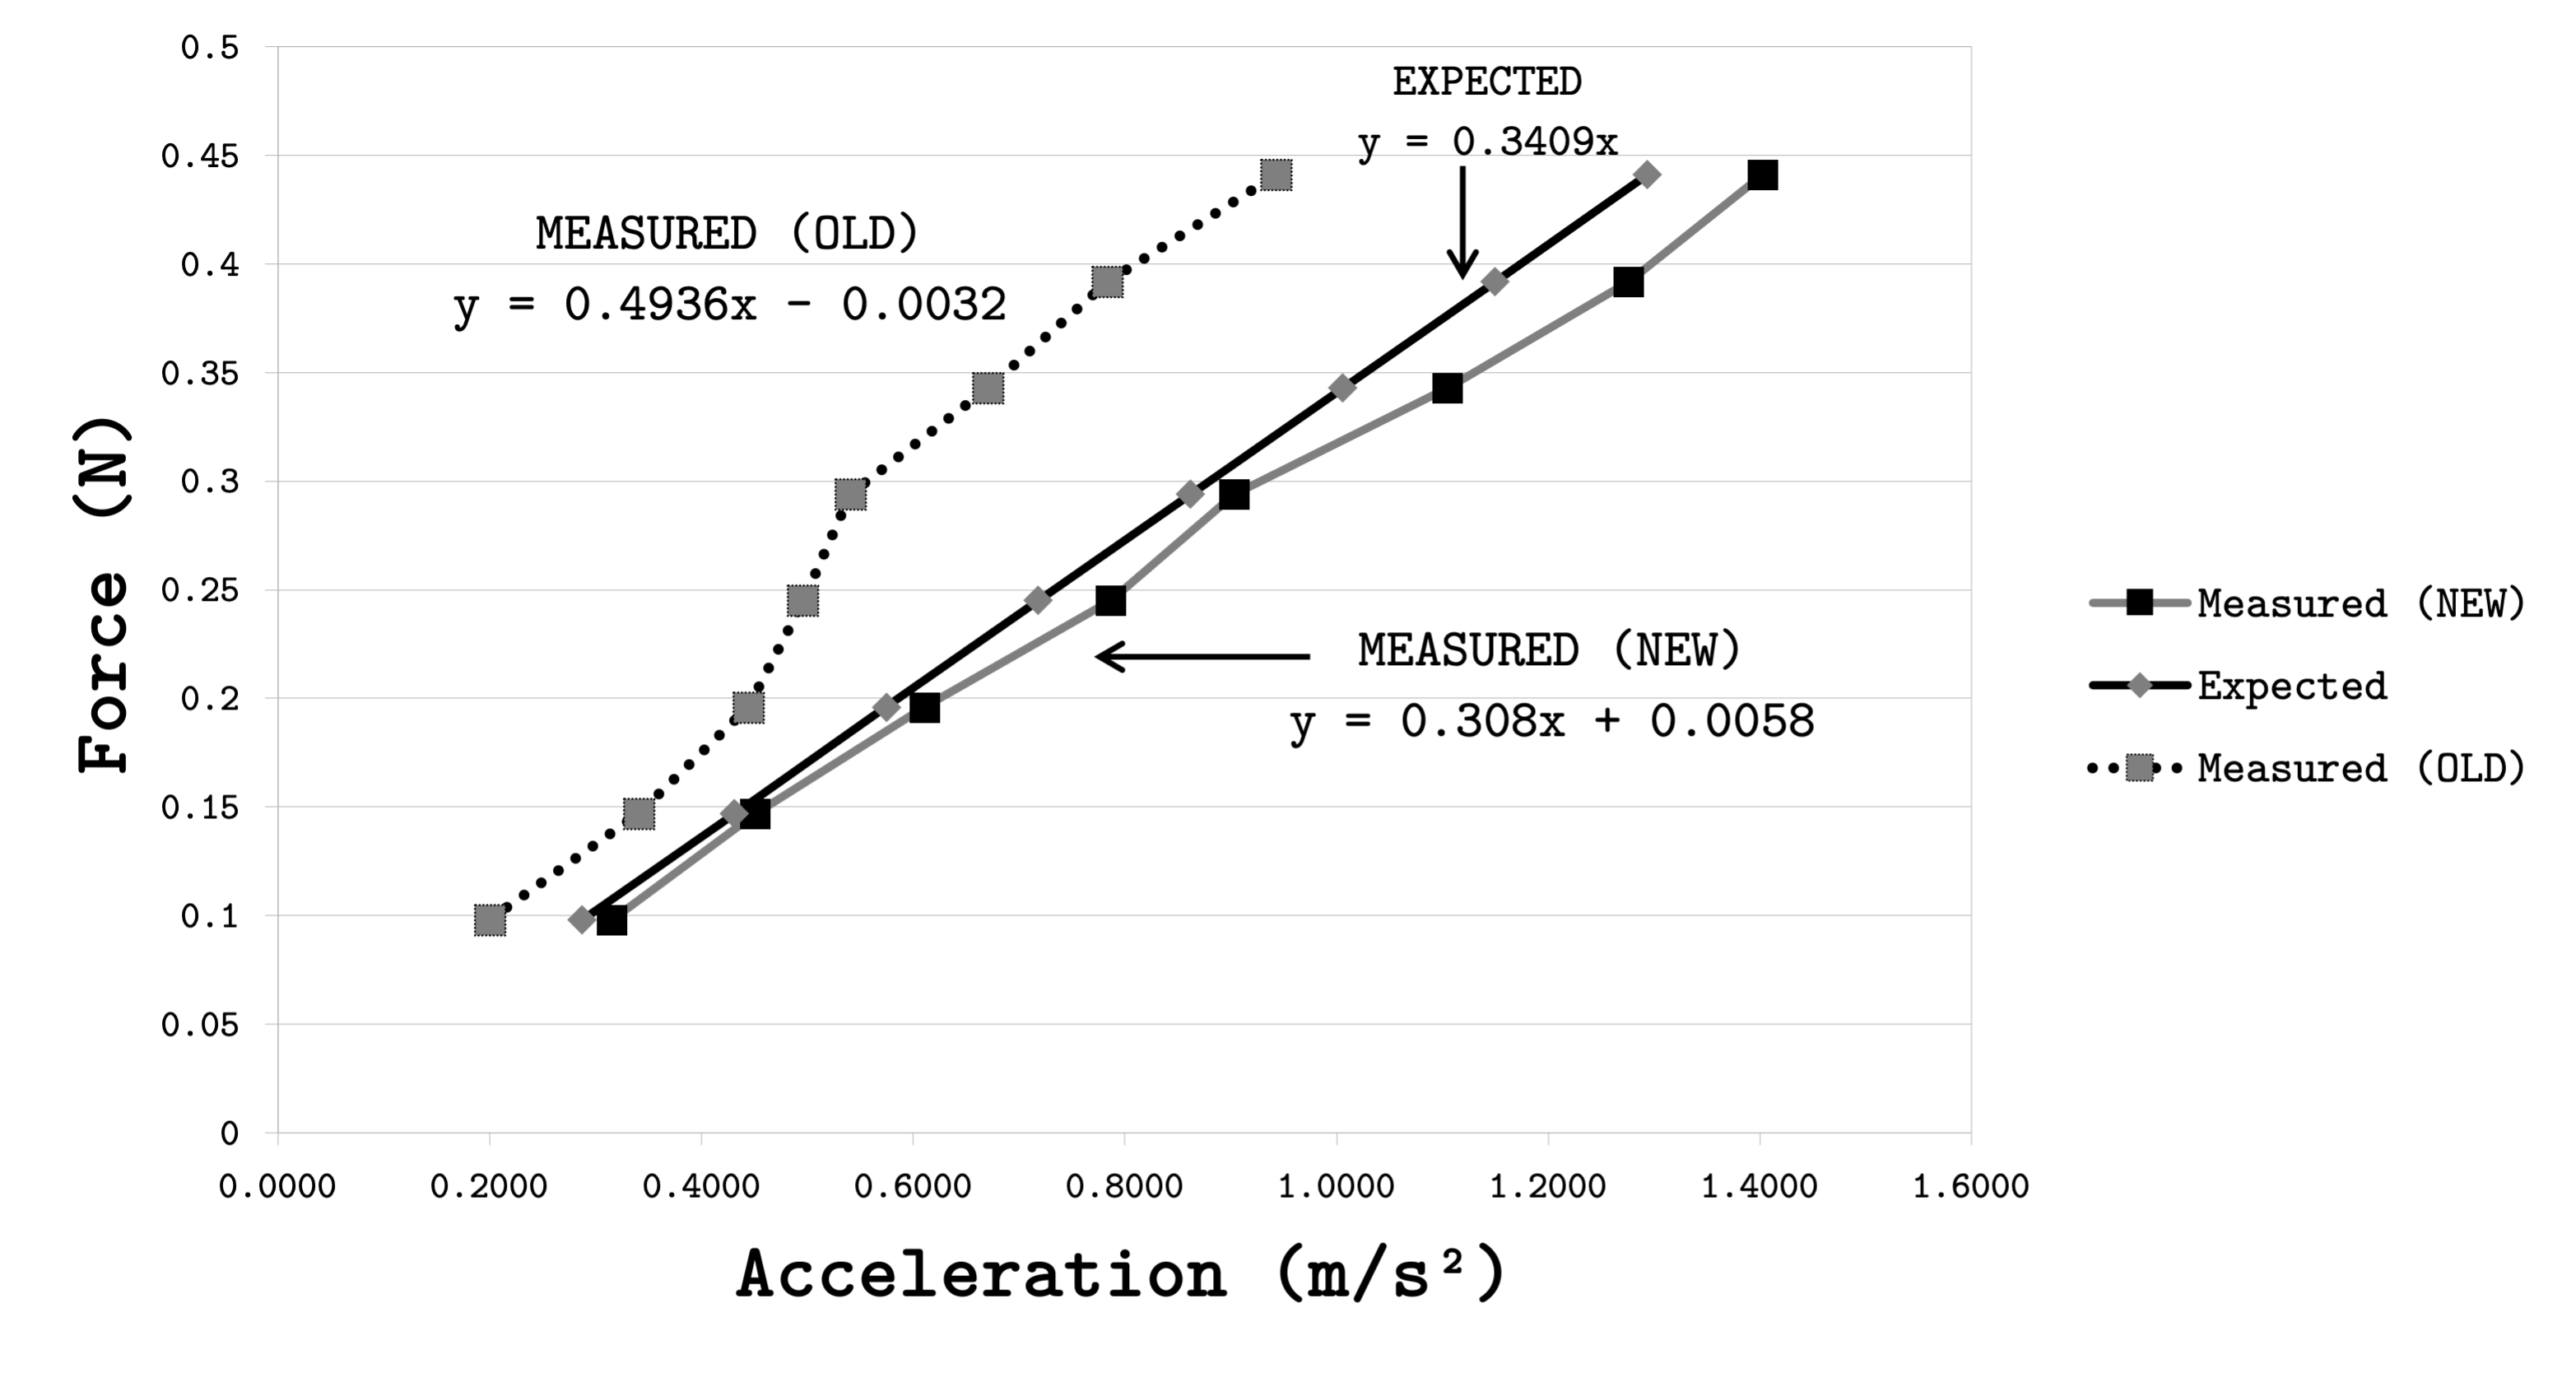
\includegraphics[width=0.90\columnwidth]{images/GraphFvA}
% 	\end{center}
% \end{figure}
% \end{landscape}

%----GRAPHS-----%

%\newpage

